

\chapter{The abstractions adequate to Chinese historical phonology}
Two abstractions govern this work, 
These two kinds of evidence imposers and transposers. 

One must distinguish two types of historical phonology, viz. the reconstruction of unattested stages of languages with the comparative method as its corresponding method and our topic—the phonological interpretation of ancient documents, or more precisely the postulation of a phonological system that in principle is associated with the speech community that produced (or altered) a particular document at a particular time, together with an interpretation of how this document instantiates this system. This second type of historical phonology, perhaps properly called `philologico-historical phonology`, also has his proper method.  Despite the dearth of secondary literature on methodology, we propose that, just as the geometer limits his tools to a straight edge and compass or the comparative linguist employs exceptionless sound change and analogy, the philologico-historical linguist also has two tools to hand, which we here call `imposition` and `transposition`. 

\section{Imposition}
Imposition is a process whereby symbols of known pronunciation in one system are brought to bear on the interpretation of symbols of unknown pronunciation in another system. By virtue of its phonetically opaque writing system Chinese furnishes a good illustration of imposition. The \textit{Menggu Ziyun} 蒙古字韻 `Rimes in Mongol Script` of 1308 provides the pronunciation of 9,118 Chinese characters in the ʼPhags-pa script. For example, for the character 農 `agriculture` it offers  which straightforwardly consists of three letters with the respective values [n], [u] and [ŋ] (Coblin 2007: 108). We are thus entitled to believe that in Beijing in 1308 the morpheme meaning `agriculture` and written 農 was pronounced /nuŋ/. As in this Chinese example, it is typically the availability of the same word in more than one writing system that permits us to impose on the language under study with a language that is already better understood. The occurrence of the name `Ptolemy` in the Greek inscriptions on the Rosetta stone and Philae obelisk is what allowed Champollion to identify this name in hieroglyphics and to associate the relevant hieroglyphs with Greek letters and thereby with phonetic values (Robinson 2012: 137 and see Fig. 1). However, the source of imposition is not necessarily itself a philological source but could be a reconstructed language. The interpretation of Mycanean q as a labiovelar is a case of imposition from a reconstruction. Mycenean qe `and` can be interpreted as /kʷe/, because *kʷe is the source of Classical Greek {\grk{τε}} that is securely reconstructible on other grounds (Latin -\textit{que}, Celtiberian -\textit{kue}, etc.). Explicit metalinguistic comments are yet another potential source for imposition. For example, the Chinese character 齈 `nasal mucus` appears on the first chart of the \textit{Yunjing} 韻鏡from 1161, under the headings dental (舌音) and resonant (清濁), which is practically speaking enough for us to know that the morpheme in question began with /n/. These examples make clear that the evidence permitting the imposition of a sound into a writing system is necessarily a material artefact that awaits discovery in the philological record, but the imposition itself—the identification of a symbol in one system with a different symbol in a different system—is a mental act on the part of a researcher.  

\section{Transposition} 
Transposition is a process whereby symbols of unknown pronunciation in a particular system are interpreted by means of symbols of known pronunciation in that same system. To take a very simple example, the spelling variation between `sulphur` and `sulfur` allows us to presume that `ph` represents the phoneme /f/. The positional complementary distribution of the Greek letters σ and ς allows us to extend the phonetic interpretation of /s/ from one to the other. Returning to Champollion`s work on Egyptian, in addition to Ptolemy, the name Cleopatra also occurs on the Philae obelisk. Four hieroglyphs are common to the two names; these appear to represent `l`, `e`, `o` and `p` (Robinson 2012: 137 and fig 2). Nonetheless, the `t` in Ptolemy and the `t` in Cleopatra are written with different signs. Champollion ignored (abstracted from) this problem, assuming that both had the same sound value /t/. In a sense Champollion here makes a mistake; today the hieroglyph �� is understood to represent /t/ [tʰ] and the hieroglyph �� represents /d/ [t] (Allen 2013: 48). If we coquette with a Hegelian mode of expression—Champolion negated the distinction between these two hieroglyphs; subsequent scholarship negated this negation, and now we recognize his `mistake` as a necessary moment of the correct understanding. 

Aside from transposing one symbol with another, as we see with �� and ��, it is also possible to employ transposition to account for an absence. Richard Bentley (1662-1742) noted anomalous hiatuses and apparent metrical problems in Homer, such as {\grk{Ἀτρεΐδης τε ἄναξ}} `and Atreides the king` in place of an expected {\grk{Ἀτρεΐδης τ`ἄναξ}} with elision (but incorrect meter).  To resolve such anomalies, Bentley proposed to add a consonant where the context requires a consonant and he restored the digamma, here {\grk{ϝάναξ}} `king`. This act of transposition is the assumption that a pattern should be extended even to contexts that at first appear exceptional. In a further application of transposition, in those words where he found reason to restore the digamma Bentley restored it in all of its occurrences. Thus, required by his digamma to change {\grk{ὕβριν ἴδῃ}} `that you may see the insolence` into {\grk{ὕβριν ϝίδῃ}}, he further amends to {\grk{ὕβριν ὁρῇς}} `id.` in order to restore the meter that his digamma has damaged. Some criticize Bentley for this overenthusiasm in restoring digammas,  but such criticism is out of place. Bentley was right to presume that a particular \textit{état de langue} either did or did not have the digamma; in holding to this principle he even anticipates the neogrammarian hypothesis. His mistake, if it can be so called, was in not uniting his perspicacious work on the digamma to his insight on the heterogenous quality of the Homeric poems (Myres 1958: 49-50). 

Turning back to Chinese, the foundational hypothesis for all work in Chinese historical phonology, the 'xiéshēng hypothesis', is also an instance of transposition. We recall that a Chinese character is typically composed of two parts, one giving an indication of sound and the other giving an indication of meaning. If we look at the series of characters built on the same phonetic component (a `xiéshēng series`), we find that a given series offers only very few rimes.  For example, in the Middle Chinese pronunciation of 602 CE the series built on 皮 (i.e. 皮 \textit{bie}, 被 \textit{bieX},  陂 \textit{pie}, 披 \textit{phie}, 跛 \textit{paX},  簸 \textit{paX}, \textit{paH}, 破 \textit{phaH}, and 婆 \textit{ba}) offers only the two rimes -\textit{a} and -\textit{ie}. In the first millennium BCE \textit{Book of Odes} the word 皮 \textit{bie} `furs` rhymes with 紽 \textit{da} `tresses` (Ode 18.1) and 陂 pie `shore` with 荷 \textit{ḫa} `lotus` (Odes 145.1); these rhymes emboldens us to speculate that the morphemes written with characters built on 皮 originally all had the same rime and thus would have rhymed in poetry composed in the language of the Odes. Duàn Yùcái 段玉裁 (1735-1815) took this conceptual step; he articulated the xiéshēng hypothesis as 同聲必同部 `same phonetic means same rime` (Li 1974-75: 221); the challenge ever since has been to propose Old Chinese reconstructions that satisfying this hypothesis and also lead to the attested Middle Chinese outcomes through regular sound change.

The three examples of transposition we have considered—Champollion`s identification of �� and ��, Bentley`s restoration of ϝ, and Duàn Yùcái`s xiéshēng hypothesis—share a parallel logical structure. In each case the researcher begins with an empirical observation and then assumes the content of this observation as a dogma that structures subsequent investigation. Note that this inducto-dogmatic structure is the opposite of Karl Popper`s hypothetico-deductive method. Popper holds that “how it happens that a new idea occurs to a man … may be of great interest to empirical psychology; but it is irrelevant to the logical analysis of scientific knowledge” (1959: 9). Instead, we find that the structure of the matter itself urges an idea upon the investigator. Nonetheless, we can agree with Popper that “an assertion which owing to its logical form is not testable can at best operate, within science, as a stimulus” (1959: 99), but only if we amend his `can at best operate` to `must operate`.  

Allen, James P. (2013). The Ancient Egyptian Language: An Historical Study. Cambridge: Cambridge University Press. doi: 10.1017/CBO9781139506090

Brandom, Robert B. (2019). A Spirit of Trust: a reading of Hegel`s Phenomenology. The Belknap Press of Harvard university Press.  

Donaldson, John William (1859). The new Cratylus. 3d ed. London: J.W. Parker.

Gastaldi, Juan L. (2021). “Why Can Computers Understand Natural Language?.” Philosophy and Technology 34, 149–214. https://doi.org/10.1007/s13347-020-00393-9

Jebb, Richard Claverhouse (1882). Bentley. London: Macmillan and Co.

Van der Kuijp, Leonard (1986). "Studies in the Life and Thought of Mkhas grub rje IV: Mkhas grub rje on Regionalisms and Dialects," Berliner Indologische Studien 2, 23-49.

Li Fang-Kuei (1974–1975). `Studies on Archaic Chinese.` Gilbert L. Mattos, trans. Monumenta Serica 31: 219–287.

Lupi, Francesco (2022). "Richard Bentley and Philology as the Art of Conjecture". In: History of Classical Philology: From Bentley to the 20th century, Diego Lanza and Gherardo Ugolini, eds. Berlin: De Gruyter, pp. 9-34. https://doi.org/10.1515/9783110730388-002

Myres, John Linton (1958). Homer and His Critics. London: Routledge and Kegan Paul. 

Mimaki, Katsumi (1990). “ウパロサル (dBus pa blo gsal) の『新旧語彙集』(brDa gsar rñiṅ gi rnam par dbye ba) 校訂本初稿Dbus pa blo gsal no `Shin Kyuu Goi Shu` –Kōteibon Shokō / A Fourteenth-Century Tibetan Lexicographical Work, the brDa gsar rñiṅ gi rnam par dbye ba by dBus pa blo gsal.” アジアの言語と一般言語学: 西田龍雄教授還暦記念論集 Ajia no gengo to ippan gengogaku: Nishida Tatsuo kyōju kanreki kinen ronshū / Asian Languages and General Linguistics, Festschrift for Prof. Tatsuo Nishida on the occasion of his 60th birthday. Tokyo: 三省堂 Sanseidō 17-54.

Miyake, M. (2018). “Studies in Pyu Phonology, ii: Rhymes”, Bulletin of Chinese Linguistics, 11(1-2), 34-76. doi: https://doi.org/10.1163/2405478X-01101008

Miyake, M. (2021). “Studies in Pyu phonology, I, Onsets”, Language and Linguistics, 22(1), 28-70. doi: https://doi.org/10.1163/2405478X-01101008

Robinson, A. (2012). Cracking the Egyptian code: the revolutionary life of Jean- Francois Champollion. London: Thames and Hudson.


\section{Structure and conventions of this book}
We start at the end, in so far as the reconstruction of Old and Middle Chinese will be taken for granted as the various relevant kinds of evidence are presented through Chinese history. 

Middle Chinese and Old Chinese will be presented exegetically as two totalities.  





\section{imposers and transposers}

Both imposers and transposers are forms of abstraction; they are equivalence relations. imposers equate a sign of one system with a sign of another system. Transposers equate two or more signs within the same sign system. 

The preservation of the Greek phrase 
{\grk{Κύριε ἐλέησον}} `lord have mercy'
 as \textit{kyrie eleison} 
  in the Latin liturgy 
 provides a clear example of an alphabetizer. The spelling of these two Greek words in Roman letters allows us to associate the graphic symbols of the two script systems into equivalents: 
 ({\grk{κ}}, k), 
 ({\grk{ύ}}, y), 
 ({\grk{ρ}}, r), 
 ({\grk{ι}}, i), 
 ({\grk{ε}}, e), 
 ({\grk{ἐ}}, e), 
 ({\grk{λ}}, l), 
 ({\grk{έη}}, ei)
 ({\grk{σ}}, s)
 ({\grk{ο}}, o)
 ({\grk{ν}}, n). 
Like any collection of ordered pairs, this set can also represented as a function. 
Thus, 
%\begin{center}
\begin{equation}
\mathfrak{f}: G \longrightarrow L 
\end{equation}
%\end{center}
where 
$\mathfrak{f}$({\grk{κ}}) = k, $\mathfrak{f}$({\grk{ρ}}) = r, etc.  
Naturally, the function 
$\mathfrak{f}$
is an interpretation of Greek letters into the Latin alphabet.\footnote{Since Greek and Roman letters are serving as elements of the domain or codomain of our functions, it seems safest to represent the functions themselves with Fraktur.} The same set of ordered pairs also yields a function 
\begin{equation}
\mathfrak{f}: L \longrightarrow G 
\end{equation}
where 
$\mathfrak{f}$(k) = {\grk{κ}}, 
$\mathfrak{f}$(r) = {\grk{ρ}}, etc.  
In other words, the data itself does not specify which alphabet is \textit{interpretandum} and which serves as \textit{interpretans}; the investigator makes this decision depending on her aims. 

The spelling variation between `sulphur' and `sulfur'  provides a clear example of a transitivizer. The association of these two spelling also yields a set of ordered pairs: (s, s), (u, u), (ph, f), (u, u), (r, r). 
These ordered pairs us a function 
\begin{equation}
\mathfrak{f}
: L \longrightarrow L 
\end{equation},
where 
$\mathfrak{f}$(s) = s, 
$\mathfrak{f}$(ph) = f, etc.



NOW I NEED TO PROVE THAT THESE SET UP AN 
equivalence relation is a binary relation that is reflexive, symmetric and transitive. The

IT ISN'T GOING TO WORK, SO WE TURN TO NETWORK THEORY INSTEAD. ALPHABETIZER IS A BIPARTITE NETWORK AND TRANSITIVIZEZR IS A NORMAL (MONOPARTITE?) NETWORK

It behooves us to explore these two abstractions at greater length before deploying them in the study of Chinese. 

EXPLAIN MY CHOICE OF EGYPTIAN AND SUMERIAN 
IN TERMS OF BRANDOM'S bimodal hylomorphic conceptual realism 

\subsection{The decipherment of Egyptian}

\begin{figure}[h]
    \centering
    \begin{tabular}{p{0.02\textwidth}p{0.06\textwidth}p{0.05\textwidth}p{0.04\textwidth}p{0.05\textwidth}p{0.07\textwidth}p{0.04\textwidth}p{0.1\textwidth}}
        &  & p &  &  & l &  & \\
        \multicolumn{8}{c}
        {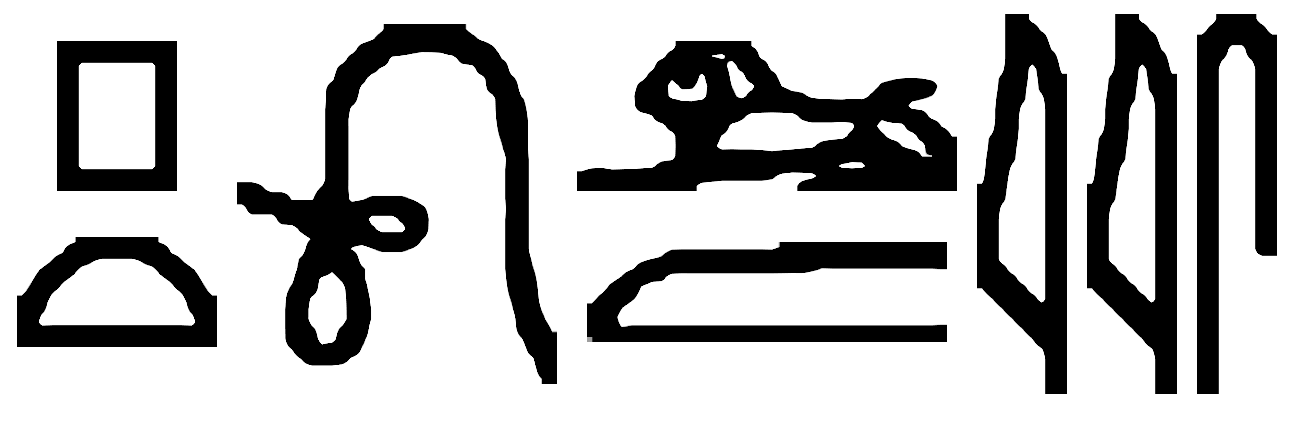
\includegraphics[scale=0.2]{Chapter1/Ptolemy.png}}
        \\
&  & t & o &  & m & e & s
  \end{tabular}
    \caption{The name Ptolemy on the Rosetta stone and the Philae obelisk 
    \citep[137]{Robinson2012Egyptian}}
    \label{fig:Ptolemy}
%\end{figure}


%\begin{figure}
%    \centering
    \begin{tabular}{p{0.05\textwidth}p{0.06\textwidth}p{0.05\textwidth}p{0.04\textwidth}p{0.05\textwidth}p{0.1\textwidth}p{0.08\textwidth}p{0.06\textwidth}}
        & c &  &  &  &  & t &   \\
        \multicolumn{8}{c}
        {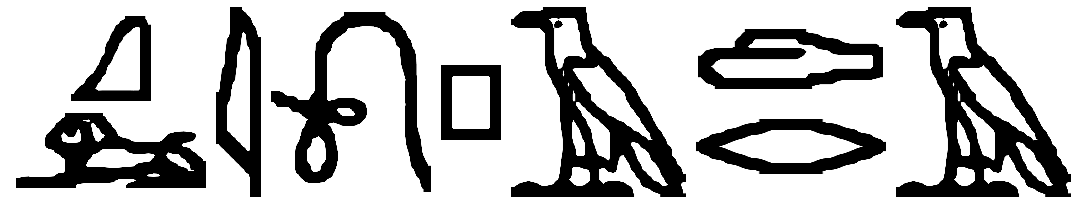
\includegraphics[scale=0.4]{Chapter1/Cleopatra2.png}}
        \\
& l & e & o & p & a & r & a
  \end{tabular}
    \caption{The names Cleopatra on the Philae obelisk 
    \citep[137]{Robinson2012Egyptian}}
    \label{fig:Cleopatra}
%\end{figure}

%\begin{figure}
%    \centering
    \begin{tabular}{p{0.04\textwidth}p{0.09\textwidth}p{0.05\textwidth}p{0.04\textwidth}p{0.06\textwidth}p{0.1\textwidth}p{0.06\textwidth}}
        && l &  &  & ?\sil{₂} & r  \\
        \multicolumn{7}{c}{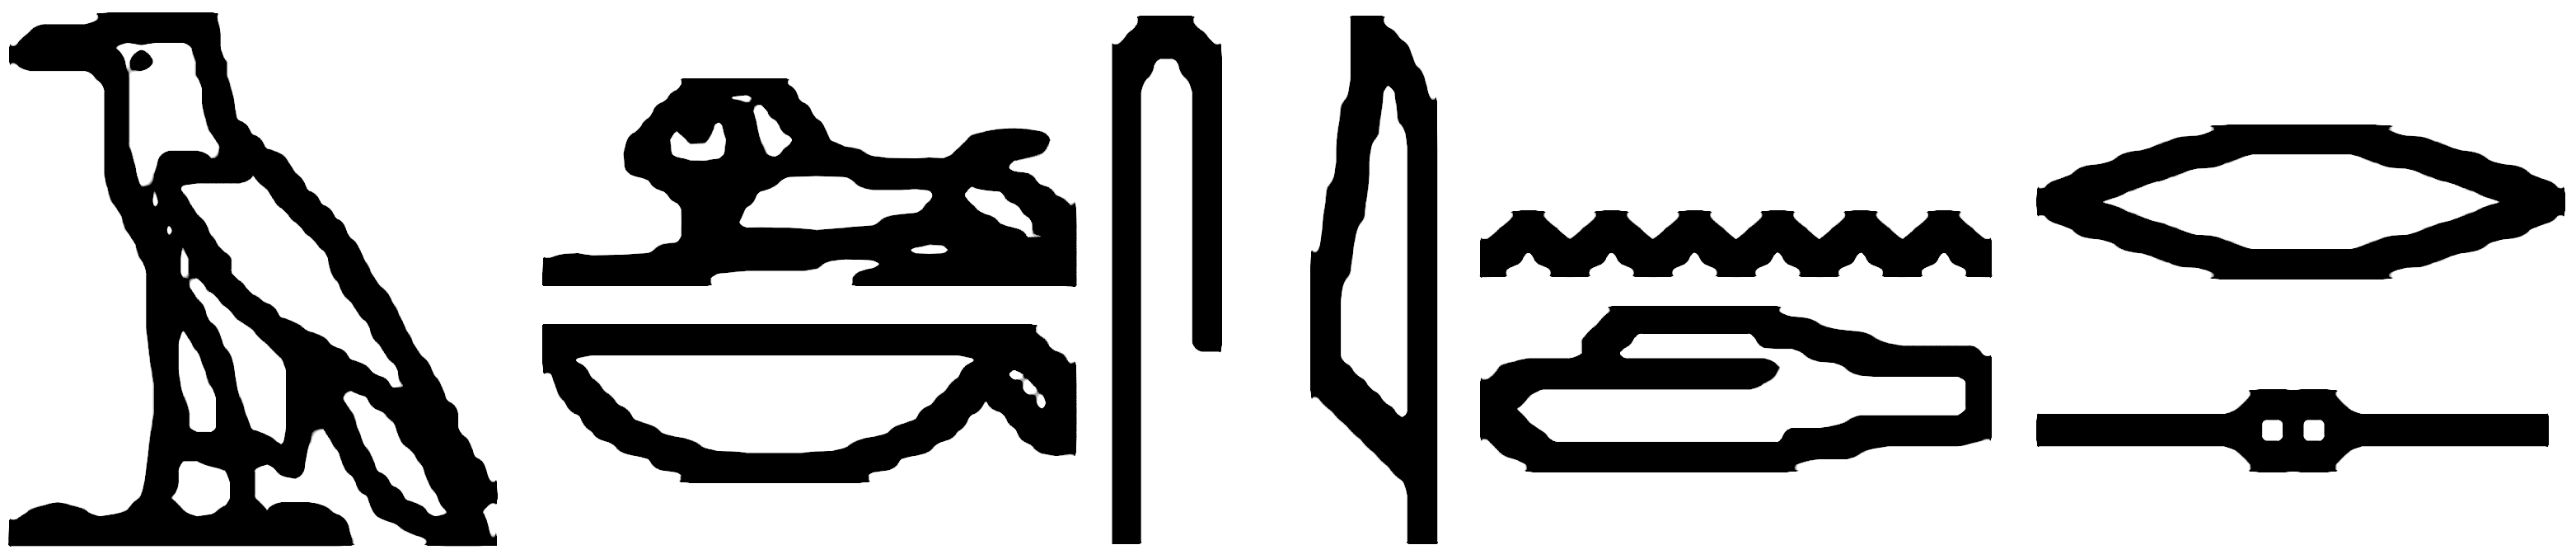
\includegraphics[scale=0.12]{Chapter1/Aleksandr.png}}
        \\
&a & ?\sil{₁} & s & e & t & ?\sil{₃} 
  \end{tabular}
    \caption{The name Alexander (\textit{Alexandros}) on the Philae obelisk 
    \citep[137]{Robinson2012Egyptian}}
    \label{fig:Alexander}
\end{figure}


The Egyptian orthographic practice of placing proper names in cartouches was the precondition for the decipherment of the language, since it allowed one to associate the Greek personal names appearing on the Rosetta stone with Egyptian equivalents. 

Although the Rosetta stone has the fame for enabling the decipherment of Egyptian. It was awareness of a second object bearing a bilingual inscription, namely the Philae obelisk, which proved decisive.\footnote{Masséglia, Jane (2020). "Imaging Inscriptions: The Kingston Lacy Obelisk". The Epigraphy of Ptolemaic Egypt. Oxford: Oxford University Press. pp. 9–19. ISBN 9780198858225. This article annoyingly doesn't include the text of the inscription. It does have a reference to the publication by Lepsius. It also mentions that the inscription has the inventory number 424 in a planned published corpus.} The name Ptolemy occurs on both objects, spelled the same way. The name Cleopatra also occurs on the Philae obelisk. In the first instance Champollion's approach to decipherment was to identify Greek letters with Egyptian hieroglyphs (see figure \ref{fig:Cleopatra}). 
Four signs are common to the two names, which appear to represent \textit{l}, \textit{e}, \textit{o} and and \textit{p}. 
The appearance of both instances of the `a' in Cleopatra as eagle sign, gives weight to their interpretation, just as was the case for four signs  \textit{l}, \textit{e}, \textit{o} and and \textit{p} appearing in both names. 
The `t' in Ptolemy and the `t' in Cleopatra are written with different signs. Champollion ignored (abstracted from) this problem, assuming that both had the same sound value /t/. 


Next we turn to 
figure \ref{fig:Alexander};
already we can read six of its nine signs.\footnote{Question: the name Alexander was in the Greek version of the inscription, right? I need to check this.}
Champollion guessed that the three relevant values were 'k','n' and 's'. Only 'n' is new to the hypothetical phonological system. Otherwise, we add new transitive relationships among the signs ({\img{Chapter1/EgyQ.png}} = {\img{Chapter1/EgyK.png}}, {\img{Chapter1/EgyS.png}} = {\img{Chapter1/EgyZ.png}}). 

Some of these relationships turn out to be wrong, but the positing of the relationships was necessary, whereas the fact that they are wrong is contingent. To put this differently, the recognition that they are wrong can only be gained from the standpoint that believes in them. 
In the first instance this is not a historical but a logical claim. 
Perhaps there is a way to move from total ignorance of Egyptian writing system to the Egyptological \textit{opinio communis} of 2022 without ever passing through Champollion's particular errors (abstractions).\footnote{One would for one thing probably start from Proto-Coptic rather than from Greek as the alphabetizer.} 
But any path would have its errors, in the sense of simplifying assumptions that serves as a scaffolding to build the theoretical edifice, which we suspend once the edifice is in place 
\citet[60-72]{Pope1999decipherment}

I need to discuss this stuff in terms of imposers and transposers and do a little pseudo-math. 

\begin{equation}
\mathfrak{f}: G \longrightarrow E 
\end{equation}
where 
$\mathfrak{f}$(t) = {\img{Chapter1/EgyT.png}}, 
$\mathfrak{f}$(p) = {\img{Chapter1/EgyP.png}}, etc.


\begin{equation}
\mathfrak{f}: E \longrightarrow E 
\end{equation}
where 
$\mathfrak{f}$({\img{Chapter1/EgyT.png}}) = {\img{Chapter1/EgyD.png}}, etc.


Ptolemaios 

{\egy{ptwꜣrwmys}}

Cleopatra

{\egy{qrwjwꜣpꜣdrꜣ}}

Alexander

{\egy{ꜣrwksjndrs}}



\subsection{The invention of writing}
In the case of Egyptian decipherment, Champollion moved from a script system, whose monuments remained available iin his own day, to the pronunciation of an ancient language. The invention of writing is a movement in exactly the opposite direction. The inventor starts from sounds already available in his speech community two written symbols made available for future generations. 

The greatest historical achievement advanced by the invention of writing is the notion of writing itself. 
In the case that a language without a previous tradition of literacy gains a writing system, the idea of writing itself is naturally already available. For Sumarian, a long historical process culminated in writing. It is more accurate to say that writing was discovered than that it was invented.

Sumerian writing begins c. 31st century BCE.\footnote{The older the texts are the more morphemes are omitted in the writing. Sumerian has is typologically exciting  have lots of prefixes and suffixes and agreement and all sorts of exciting stuff going on all the type that we have in a lot of languages like early 2nd Millennium when Sumerian was probably already extinct and only spoken in schools that all of the affixes are fully expressed which is to say if you look at the early Sumerian when Sumerian was a robust living language from the point of view of an investigator today it might well look like a highly isolating language with very little morphology and that's just because the samarians didn't feel the need to write it down because they all knew it whereas in particular in this bilingual context of  Akkadians having to learn Sumerian as a second language they felt the need to spell everything out. 
This is a useful no story to keep in mind. Apparently isolating graphic information does not necessarily say anything about what the morphological profile of the language was. The following observations are worth keeping in mind in the context of morphology in old Chinese, but they are not directly relevant here.  ``the older the texts the more morphemes are omitted in the writing'' (Thomsen 1984: 28 qtd. in Handel 2019: 287). ``in the early second millennium, when Sumerian
was probably extinct and spoken only in the schools, are the affixes fully
expressed'' (Cooper 1996: 43).} For our present purposes the detailed stages that lead up to writing itself are not relevant.\footnote{GIVE SOME DETAIL AND CITATIONS}. Instead, here it suffices to present the matter as is the inventor of the Sumerian script had a specific goal in mind.

\begin{figure}[h]
\begin{center}
\begin{tabular}{cc}
\begin{tabular}{c}
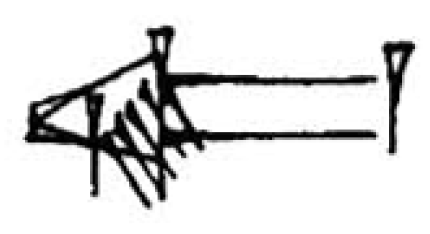
\includegraphics[scale=0.5]{Chapter1/ka2.png}     
\end{tabular}
& {\Large {ka}} `mouth'       \\
\begin{tabular}{c}
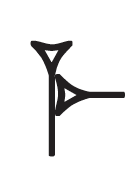
\includegraphics[scale=0.6]{Chapter1/ME2.png}     
\end{tabular}
& {\Large {me}} `hundred'       \\
\begin{tabular}{c}
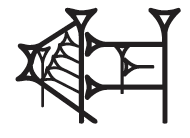
\includegraphics[scale=1.2]{Chapter1/eme.png}     
\end{tabular}
& {\Large {eme}} `tongue'       \\

\end{tabular}

\end{center}
    \caption{The Sumerian signs for \textit{ka} `mouth', \textit{me} `hundred'  and \textit{eme} `tongue'.}
    \label{fig:Sumerian-eme}
\end{figure}

We begin our tale when the Sumerians had already invented signs for certain \textit{realia} (body parts, animals, grains) and for numbers. For example, a sign for \textit{ka} `mouth' and a sign for \textit{me} `hundred'.  
When possessed of the design to, for the first time, write the word \textit{eme} `tongue' our Sumerian chose to put the sign for \textit{me} `hundred' inside of the sign for \textit{ka} `mouth'. 
He expected his readers to recognize both signs in this novel combination, posing themselves the question `what is a word that means something like `mouth'  and sounds something like \textit{me}?',  and using their own native-speaker knowledge of the language to come immediately to the answer \textit{eme} `tongue' (see figure \ref{fig:Sumerian-eme}).\footnote{If the reader instead posed the question `what is a word that means something like `hundred' and sounds something like \textit{ka}?', not coming upon any obvious word, would move immediate on to asking the right question, especially when aided by the overall context of the document, which would provide a context in which `tongue' made good sense.} 
This process of creating new graphic signs is, as we shall see anon, the exact analogy of how the phonosemantic (形聲) characters of Chinese were formed. 

Let us consider a second  example 
We now find ourselves wanting to write the word \textit{nundum} `lip'. 
We start again with \textit{ka} `mouth' but this time we put \textit{nun} `prince'  inside of it we then get a \textit{nundum}
`lip', a word that has something semantically to do with `mouth' and something phonetically to do with \textit{nun} (\ref{fig:Sumerian-nundum}. 

\begin{figure}[h]
\begin{center}
\begin{tabular}{cc}
\begin{tabular}{c}
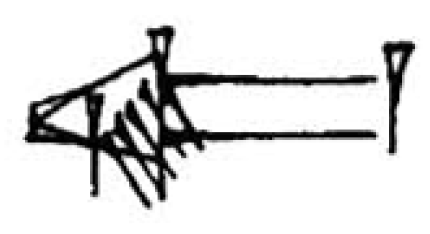
\includegraphics[scale=0.5]{Chapter1/ka2.png}     
\end{tabular}
& {\Large {ka}} `mouth'       \\
\begin{tabular}{c}
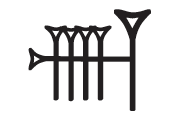
\includegraphics[scale=0.6]{Chapter1/nun.png}     
\end{tabular}
& {\Large {nun}} `prince'       \\
\begin{tabular}{c}
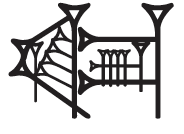
\includegraphics[scale=1.2]{Chapter1/nundum.png}     
\end{tabular}
& {\Large {nundum}} `lip'       \\

\end{tabular}

\end{center}
    \caption{The Sumerian signs for \textit{ka} `mouth', \textit{nun} `prince'  and \textit{nundum} `lip'.}
    \label{fig:Sumerian-nundum}
\end{figure}

Let us now develop some abstractions about how Sumerian works. 
A particular grapheme is associated with at least one semantic value and one phonetic value. 
Using a notation that William Bolts puts forward, we may thus symbolize a grapheme as G a set \{S, P\}. 
When we combine two graphemes in order to coin a fresh one, we, in the first instance thus bring together a grapheme G₁ = \{S₁, P₁\} and a grapheme G₂ = \{S₂, P₂\}. We now ignore the phonetics of G₁ and the semantics of  G₂ in order to form 
G₃ = \{S₁, P₂\}. 


If we want to conceptualize the creation of new graphemes in terms of abstractions. We have two, which we may for the moment call `semantic extension' and `the Rebus principle'. 

\begin{equation}
S: \{S_1, P_1\} \rightarrow \{S_1\} 
\end{equation}

\begin{equation}
R: \{S_2, P_2\} \rightarrow \{P_2\} 
\end{equation}
Of course, G₃ does not in fact have semantics S₁ and the pronunciation of P₂. 
The grapheme 
{\img{Chapter1/nundum.png}} 
is not \textit{nun} `mouth' but \textit{nundum} `lip. 
We should note that the map from `mouth' to `lip'  cannot be made without the aid of the G₂  \textit{nun} and likewise the map from \textit{nun} to \textit{nundum} cannot be made without the aid of the grapheme G₁.  As such, a more precise formulation is. 

\begin{equation}
S_{G_2}: \{S_1, P_1\} \rightarrow \{S_3\} 
\end{equation}

\begin{equation}
R_{G_1}: \{S_2, P_2\} \rightarrow \{P_3\} 
\end{equation}

I think we need one more equation. 

\begin{equation}
S_{G_2}R_{G_1}: \{S_1, P_1\}  \times 
 \{S_2, P_2\} \rightarrow 
\{S_3, P_3\} 
\end{equation}

I am not sure if I have this formulated quite correctly. 

The reason I am making this point is that it is only hear that we see how S is a transitivizer. It is S that allows us to pass from P2 to P3. It is only S that tells us that P2 and P3 are similar \textit{but not necessarily the same}. 

Now we are left only to observe that we have now met for a second time the same abstractions that served us in the case of the decipherment of Egyptian. 
The Rebus principle is the alphabetizer; it is the means by which the pronunciation of one morpheme is associated with the pronunciation of another.  The semantic extension is the transitivizer because it is what allows us to pass in writing from one morpheme to another.  
Recall that that in this case our words are known and the way to write them is unknown, whereas in Egyptian it was the writing that was known but not the pronunciation or meaning of the morphemes this writing system encodes. Semantic extension in essence is simply a mechanism for multiplying signs. 

\section{The continuity of history}

In his review, Gao Yong'an,\footnote{https://www.sohu.com/a/253907850_488532} like Harbsmeier, basically rejects the continuity of history as a methodological principle. Hard to find a good quote, maybe this is not the right place to mention it anyhow. 

\begin{quote}
Are we entitled to assume for
any reconstructed proto-language that no deep systemic changes relevant to our
explanation occurred in the course of those 3,000 years?
\end{quote}

One might as well ask a Greek geometer what entitles him to use a straight edge and compass. It is really just Okham's razon that we are applying here. 


{Phonetic information from external sources}
\begin{itemize}
    \item Loans from Chinese 
    \item Loans into Chinese 
    \item Explicit comments on pronunciation
\end{itemize}







{Explicit comments on pronunciation}



{Falling tone was a glottal stop}
義淨 Yìjìng (635–713 CE) in his 南海寄歸內法 Nánhǎi jìguī nèifǎ, reamrks that that characters used to transliterate short vowels in Sanskrit 皆須上聲讀之 ``should all be read in the rising tone'' (Mei 1970: 90), regardless of a character's normal reading.


{Dialect evidence for consonant clusters}
%Examples of two characters writing words typically written with one also
%appear in texts more recent that the \emph{Odes}. For example, 
The
說文解字 \emph{Shuōwén jiězì} (100 CE) says of the characters 聿
(31-18a) and 筆~(31-18d):

  

\hspace{5mm} 聿 (*[m.]rut > *lut > 
 \emph{ywit}):\\
\hspace{5mm} 所以書也 \hspace{6mm} `that with which one writes'\\
\hspace{5mm} 楚謂之聿 \hspace{6mm} `In Chǔ, it is called 聿 *[m.]rut.'\\
\hspace{5mm} 吳謂之不律 \hspace{3mm} `In Wú, it is called 不律 *pə.{[}r]ut.'\\
\hspace{5mm} 燕謂之弗 \hspace{6mm} `In Yān, it is called 弗 *put.'\\
\hspace{5mm} 筆 (*p.{[}r]ut > *prut > 
 \emph{pit}): \\
\hspace{5mm} 秦謂之筆 \hspace{6mm} `In Qín, it is called 筆 *p{[}r]ut' \\ %(cf. \cite[43]{Baxter2014OldChinese})

  

The variation among 弗 *put, 筆 *prut, and 不律 *pə.rut is good evidence
for `tight' versus `loose' clusters

%; in particular, the equation of the
%single character word 聿 `brush' with the two character spelling 不律
%strongly suggests the articulation of two distinct vowels in this
%word.\footnote{Nonetheless, in this case the `loose' versus `tight'
%  distinction is one of dialect, suggesting that all three
%  pronunciations descend from a common ancestor, i.e. although evidence
%  of Old Chinese complex onsets, this passage does not serve as evidence
%  of a `loose' versus `tight' distinction existing within a single
%  synchronic system. Perhaps the people of Wú pronounced all their
%  pre-initials loose and the people of Qín pronounced all of their
%  pre-initials tight.}


{Dialect evidence for consonant clusters}
Comment in the 顏氏家訓  \emph{Yán shì jiā xùn} by \\ 顏之推 Yán Zhītuī (531--591 CE)

  

窮訪蜀土, 呼粒{[}lip]為逼, {[}pik]時莫之解。吾云: `《三蒼》、《説文》, 此字白 下為匕, 皆訓粒。《通俗文》音方力反{[}pik]。'眾皆歡悟

  

I have exhaustively visited {[}the] Shǔ 蜀 region, and they pronounce
粒 lì {[}MC \emph{lip} `grain, particle'] as 逼 bī {[}MC \emph{pik}
`compel']; but at the time they had no way to explain it. I said: ``In
the \emph{Sān cāng} 《三倉》and the \emph{Shuōwén} 《說文》, this word
is written with 白 bái above and 匕bǐ below {[}i.e., as 皀], and is
glossed in both cases as 粒 \emph{lì }{[}`grain, particle']. The
 \emph{Tōngsú wén} 《通俗文》 gives its pronunciation as 方力切
{[} \emph{p}(\emph{jang}) + (\emph{l})\emph{ik} = \emph{pik}].'' They
were all delighted to discover this. 
%\citep[307 and 406 note 113]{Baxter2014OldChinese}.


{Dialect evidence for final *-r}
%Baxter and Sagart (2014a: 264-267) cite evidence from discussions by early Chinese writers suggesting the need to reconstruct the readings of three characters with final *r. By way of example, 
In his commentary on Lǚshì Chūnqiū 呂氏春秋 the late Hàn commentator Gāo Yòu 高誘 (fl. 205–212) wrote: 

  

今兖州人謂殷氏皆曰衣
\\ "Nowadays the people of Yǎnzhōu 兖州 all pronounce the family name 殷 Yīn [*ʔər] as 衣 Yī [*ʔ(r)əj]" %(Baxter \& Sagrat 2014: 265).






{Rhyme patterns}
    
    \begin{quotation}
采采芣苢、cǎi cǎi fóu yǐ\\
薄言采之。bó yán \textbf{CǍI} zhī\\
采采芣苢、cǎi cǎi fóu yǐ\\
薄言有之。bó yán \textbf{YǑU} zhī\\
  
采采芣苢、cǎi cǎi fóu yǐ\\
薄言掇之。bó yán DUŌ zhī\\
采采芣苢、cǎi cǎi fóu yǐ\\
薄言捋之。bó yán LUŌ zhī\\
  
采采芣苢、cǎi cǎi fóu yǐ\\
薄言袺之。bó yán JIÉ zhī\\
采采芣苢、cǎi cǎi fóu yǐ\\
薄言襭之。bó yán XIÉ zhī\\
%  

%\noindent Colorful is the plantain, we gather it;\\
%colorful is the plantain, we hold it.

%  
%\noindent Colorful is the plantain, we pick it;\\
%colorful is the plantain, we pluck it.

%  
%\noindent Colorful is the plantain, we take it in our held-up flaps;\\
%colorful is the plantain, we take it in our tucked-up flaps.\\
\end{quotation}






%Let's look at some Sumerian concretely. This is the sign for the word sag, which means `head'. Later it was written like this. You can see that it goes from more iconic to more abstract, partly just for reasons of the convenience of writing. Here is the sign for mouth so you see it's it's like the sign for `head' but with some indication that you should pay attention to this particular part. This sign also stylized in a way that has a certain graphic relationship to the stylized version of head but no phonetic relationship. 
